\begin{figure}[htb]
\centering
\includegraphics[page=8,width=0.33\textwidth]{\FCNCFigures/tthML/showFake/faketau/postfit/NOMINAL/reg1l2tau1bnj_os/BDTG_test.pdf}
\put(-40, 90){\textbf{(a)}}
\includegraphics[page=8,width=0.33\textwidth]{\FCNCFigures/tthML/showFake/faketau/postfit/NOMINAL/reg1l2tau1bnj_os/dphitauetmiss.pdf}
\put(-40, 90){\textbf{(b)}}
\includegraphics[page=8,width=0.33\textwidth]{\FCNCFigures/tthML/showFake/faketau/postfit/NOMINAL/reg1l2tau1bnj_os/drlbditau.pdf}
\put(-40, 90){\textbf{(c)}}
\\
\includegraphics[page=8,width=0.33\textwidth]{\FCNCFigures/tthML/showFake/faketau/postfit/NOMINAL/reg1l2tau1bnj_os/drlb.pdf}
\put(-40, 90){\textbf{(d)}}
\includegraphics[page=8,width=0.33\textwidth]{\FCNCFigures/tthML/showFake/faketau/postfit/NOMINAL/reg1l2tau1bnj_os/drltau.pdf}
\put(-40, 90){\textbf{(e)}}
\includegraphics[page=8,width=0.33\textwidth]{\FCNCFigures/tthML/showFake/faketau/postfit/NOMINAL/reg1l2tau1bnj_os/drtaub.pdf}
\put(-40, 90){\textbf{(f)}}
\\
\includegraphics[page=8,width=0.33\textwidth]{\FCNCFigures/tthML/showFake/faketau/postfit/NOMINAL/reg1l2tau1bnj_os/drtaujmin.pdf}
\put(-40, 90){\textbf{(g)}}
\includegraphics[page=8,width=0.33\textwidth]{\FCNCFigures/tthML/showFake/faketau/postfit/NOMINAL/reg1l2tau1bnj_os/drtautau.pdf}
\put(-40, 90){\textbf{(h)}}
\includegraphics[page=8,width=0.33\textwidth]{\FCNCFigures/tthML/showFake/faketau/postfit/NOMINAL/reg1l2tau1bnj_os/etamax.pdf}
\put(-40, 90){\textbf{(i)}}
\\
\includegraphics[page=8,width=0.33\textwidth]{\FCNCFigures/tthML/showFake/faketau/postfit/NOMINAL/reg1l2tau1bnj_os/etmiss.pdf}
\put(-40, 90){\textbf{(j)}}
\includegraphics[page=8,width=0.33\textwidth]{\FCNCFigures/tthML/showFake/faketau/postfit/NOMINAL/reg1l2tau1bnj_os/lep_pt_0.pdf}
\put(-40, 90){\textbf{(k)}}
\includegraphics[page=8,width=0.33\textwidth]{\FCNCFigures/tthML/showFake/faketau/postfit/NOMINAL/reg1l2tau1bnj_os/met_sigma.pdf}
\put(-40, 90){\textbf{(l)}}
\\
\caption{ Comparison of the variables distributions for the background and merged tuH signal in the $t_l\thadhad$. Only statistical uncertainties are being shown. Underflow and overflow bins are included respectively in the first and last bins.The real tau contributions shown from ttbar and other MC including diboson, single top, and V+jets.}
\label{fig:var_reg1l2tau1bnj_os_1}
\end{figure}
\begin{figure}[htb]
\centering
\includegraphics[page=8,width=0.33\textwidth]{\FCNCFigures/tthML/showFake/faketau/postfit/NOMINAL/reg1l2tau1bnj_os/mjjmin.pdf}
\put(-40, 90){\textbf{(a)}}
\includegraphics[page=8,width=0.33\textwidth]{\FCNCFigures/tthML/showFake/faketau/postfit/NOMINAL/reg1l2tau1bnj_os/mtaujmin.pdf}
\put(-40, 90){\textbf{(b)}}
\includegraphics[page=8,width=0.33\textwidth]{\FCNCFigures/tthML/showFake/faketau/postfit/NOMINAL/reg1l2tau1bnj_os/mtw.pdf}
\put(-40, 90){\textbf{(c)}}
\\
\includegraphics[page=8,width=0.33\textwidth]{\FCNCFigures/tthML/showFake/faketau/postfit/NOMINAL/reg1l2tau1bnj_os/nljet.pdf}
\put(-40, 90){\textbf{(d)}}
\includegraphics[page=8,width=0.33\textwidth]{\FCNCFigures/tthML/showFake/faketau/postfit/NOMINAL/reg1l2tau1bnj_os/phicent.pdf}
\put(-40, 90){\textbf{(e)}}
\includegraphics[page=8,width=0.33\textwidth]{\FCNCFigures/tthML/showFake/faketau/postfit/NOMINAL/reg1l2tau1bnj_os/t1vismass.pdf}
\put(-40, 90){\textbf{(f)}}
\\
\includegraphics[page=8,width=0.33\textwidth]{\FCNCFigures/tthML/showFake/faketau/postfit/NOMINAL/reg1l2tau1bnj_os/t2vismass.pdf}
\put(-40, 90){\textbf{(g)}}
\includegraphics[page=8,width=0.33\textwidth]{\FCNCFigures/tthML/showFake/faketau/postfit/NOMINAL/reg1l2tau1bnj_os/tau_pt_0.pdf}
\put(-40, 90){\textbf{(h)}}
\includegraphics[page=8,width=0.33\textwidth]{\FCNCFigures/tthML/showFake/faketau/postfit/NOMINAL/reg1l2tau1bnj_os/tau_pt_1.pdf}
\put(-40, 90){\textbf{(i)}}
\\
\includegraphics[page=8,width=0.33\textwidth]{\FCNCFigures/tthML/showFake/faketau/postfit/NOMINAL/reg1l2tau1bnj_os/tautauvispt.pdf}
\put(-40, 90){\textbf{(j)}}
\includegraphics[page=8,width=0.33\textwidth]{\FCNCFigures/tthML/showFake/faketau/postfit/NOMINAL/reg1l2tau1bnj_os/ttvismass.pdf}
\put(-40, 90){\textbf{(k)}}
\caption{ Comparison of the variables distributions for the background and merged tuH signal in the $t_l\thadhad$. Only statistical uncertainties are being shown. Underflow and overflow bins are included respectively in the first and last bins. The real tau contributions shown from ttbar and other MC including diboson, single top, and V+jets.}
\label{fig:var_reg1l2tau1bnj_os}
\end{figure}
